\section{App's interface accessed via Google Chrome on an Android device}
 \label{Appendixapp}

        
        
        \begin{figure}[label={fig:herokugvd}, caption={GVD-App accesed via Google Chrome in an Android device.}]
        \centering
        \begin{tabular}[c]{cc}
        \centering
        \fbox{
        \begin{subfigure}[b]{.5\textwidth}
		    \centering	
            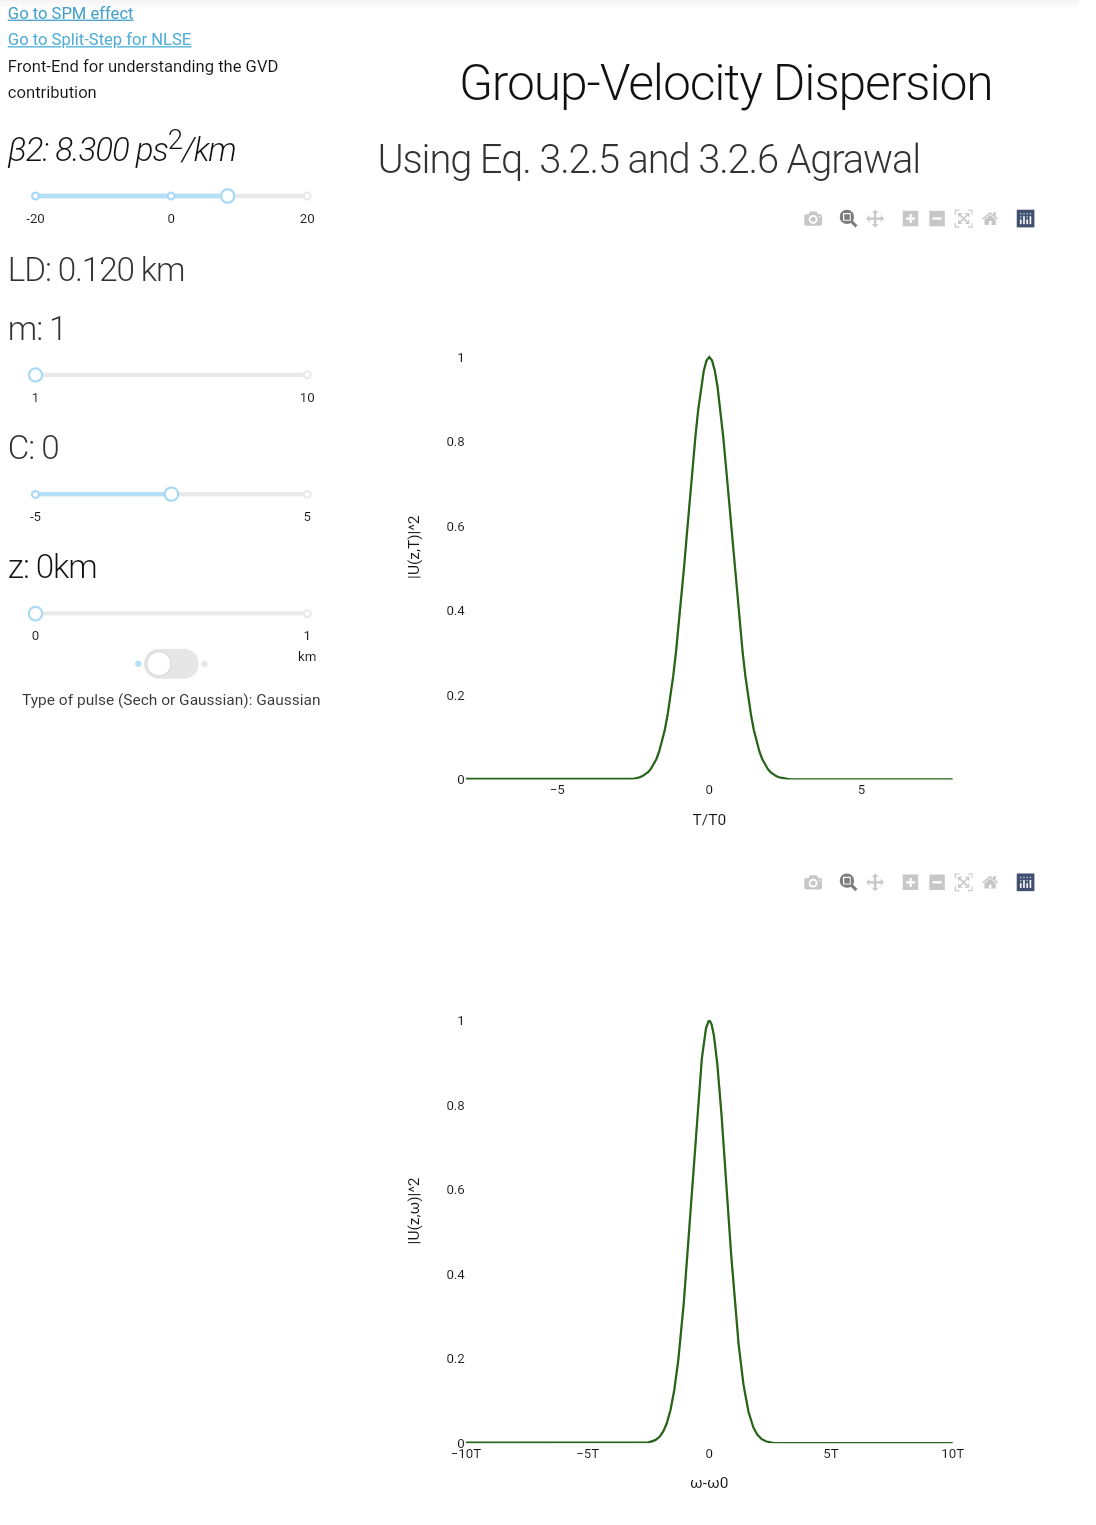
\includegraphics[width=1\textwidth]{figures/chap4/android_gvd1.png}
            \caption{First part of the GVD-app.}
            \label{fig:herokugvd1}
        \end{subfigure}}
        \hfill
        \fbox{
        \begin{subfigure}[b]{.5\textwidth}
		    \centering	
            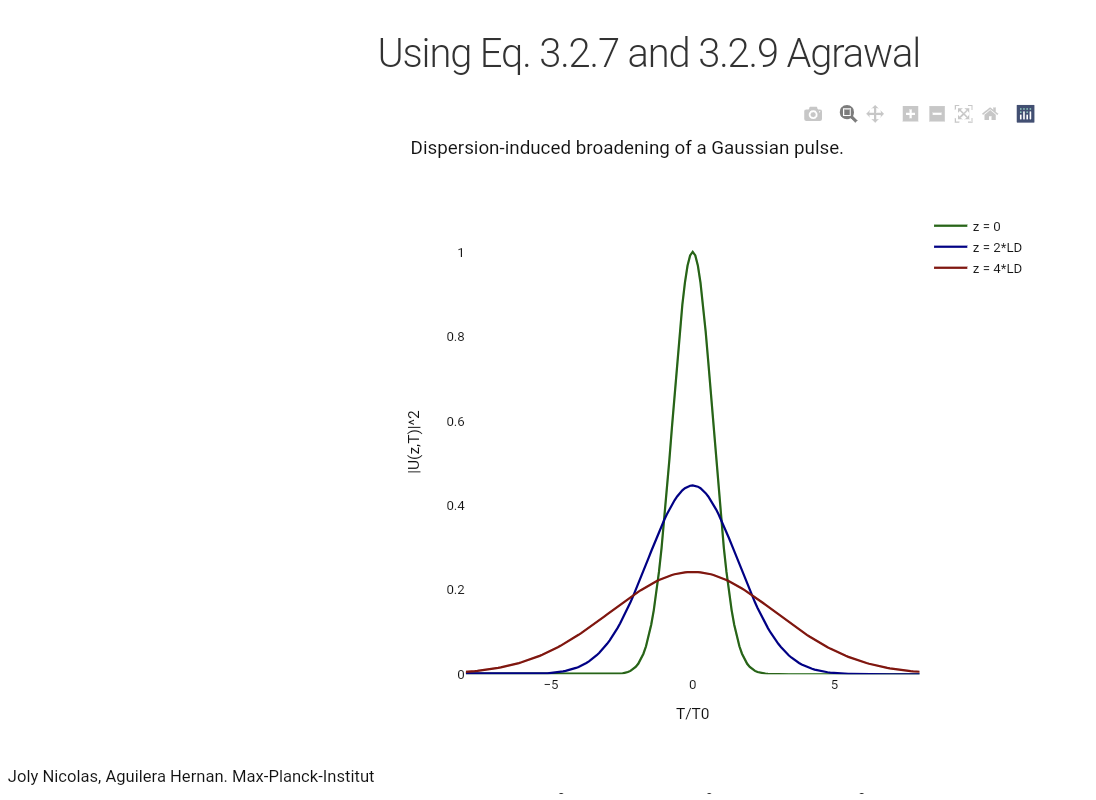
\includegraphics[width=1\textwidth]{figures/chap4/android_gvd2.png}
            \caption{Second part of the GVD-app.}
            \label{fig:herokugvd2}
        \end{subfigure}}
        \end{tabular}
        \end{figure}
        
        \begin{figure}[label={fig:herokuspm}, caption={SPM-App accesed via Google Chrome in an Android device.}]
          %  \caption*{Source: Some Source}
          \fbox{
        	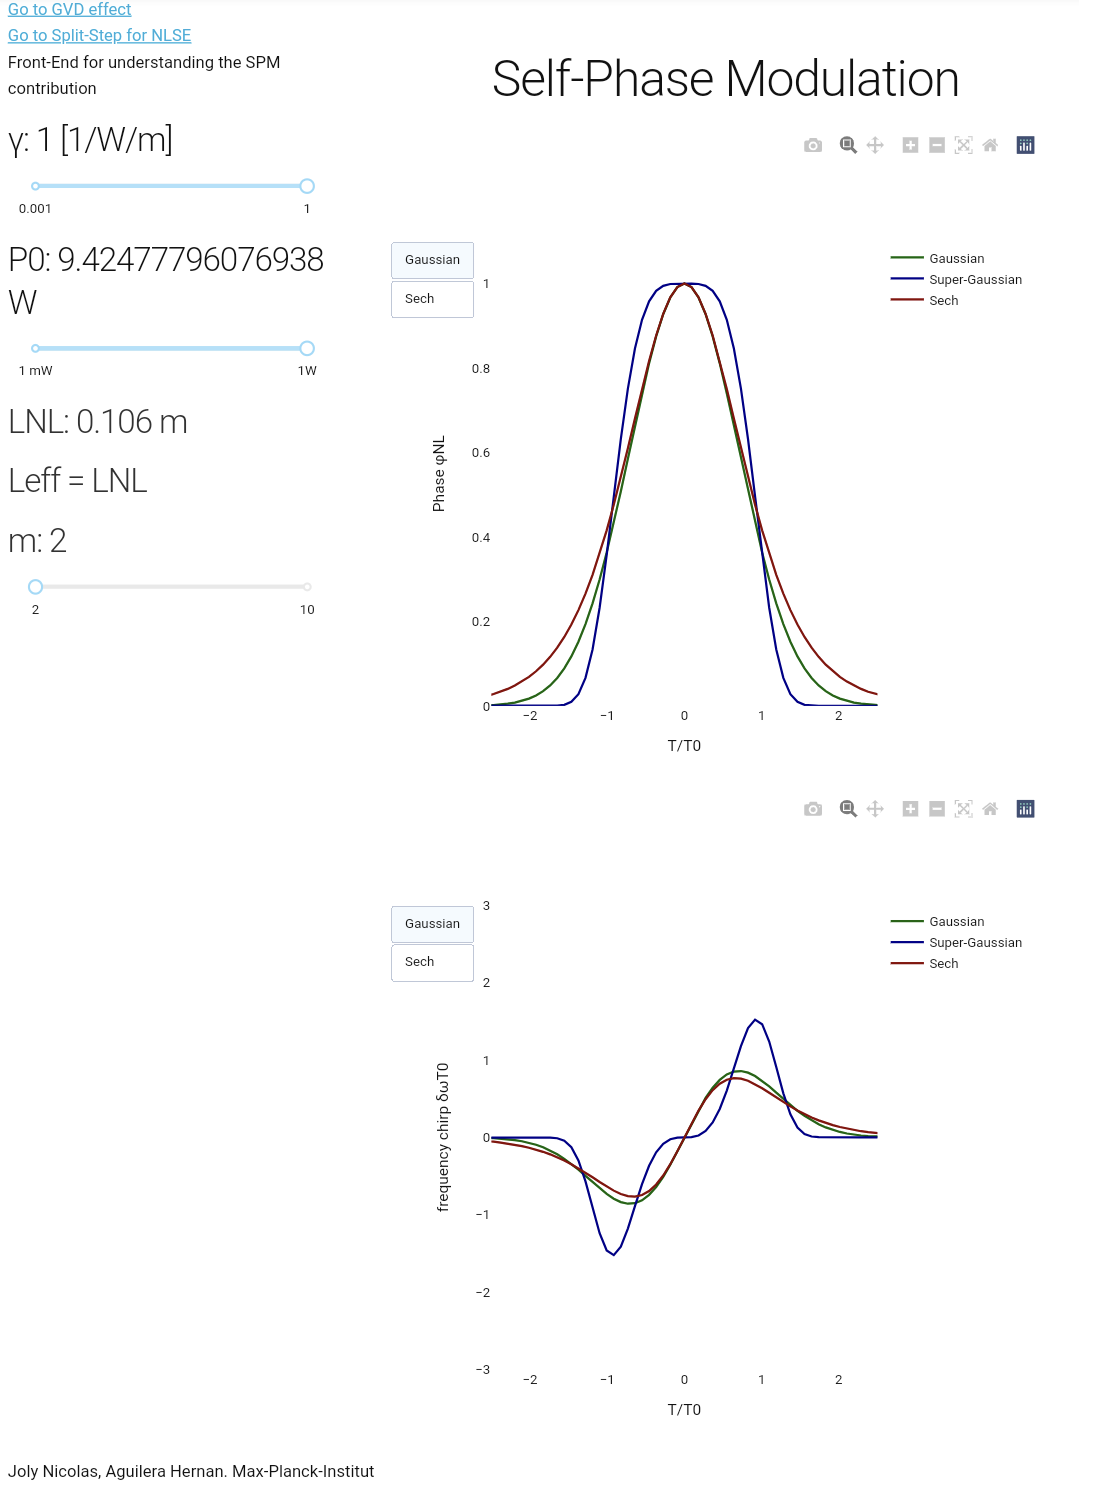
\includegraphics[width=.8\textwidth]{figures/chap4/android_spm.png}} 
        \end{figure}
        

    \begin{figure}[label={fig:herokunlse}, caption={NLSE-App accesed via Google Chrome in an Android device.}]
        \centering
        
        \begin{tabular}[c]{cc}
        \centering
        \fbox{
        \begin{subfigure}[b]{.5\textwidth}
		    \centering	
            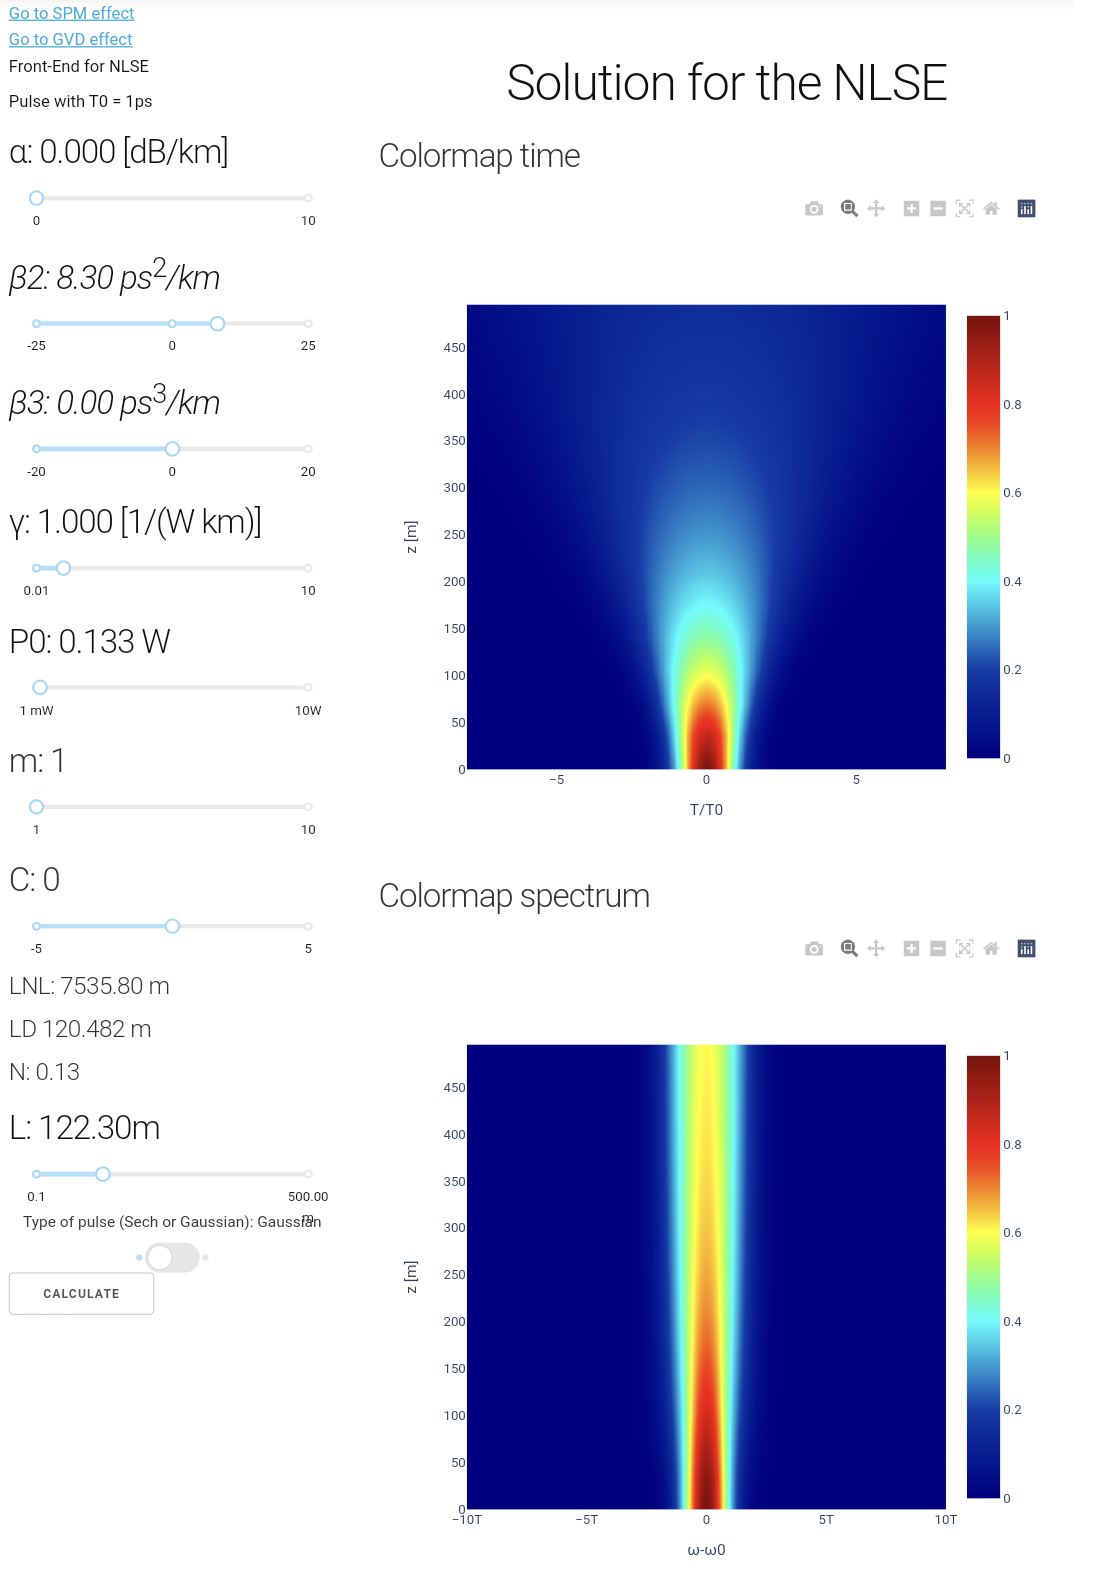
\includegraphics[width=1\textwidth]{figures/chap4/android_nlse1.png}
            \caption{First part of the NLSE-app.}
            \label{fig:herokunlse1}
        \end{subfigure}}
        \hfill
        \fbox{
        \begin{subfigure}[b]{.48\textwidth}
		    \centering	
            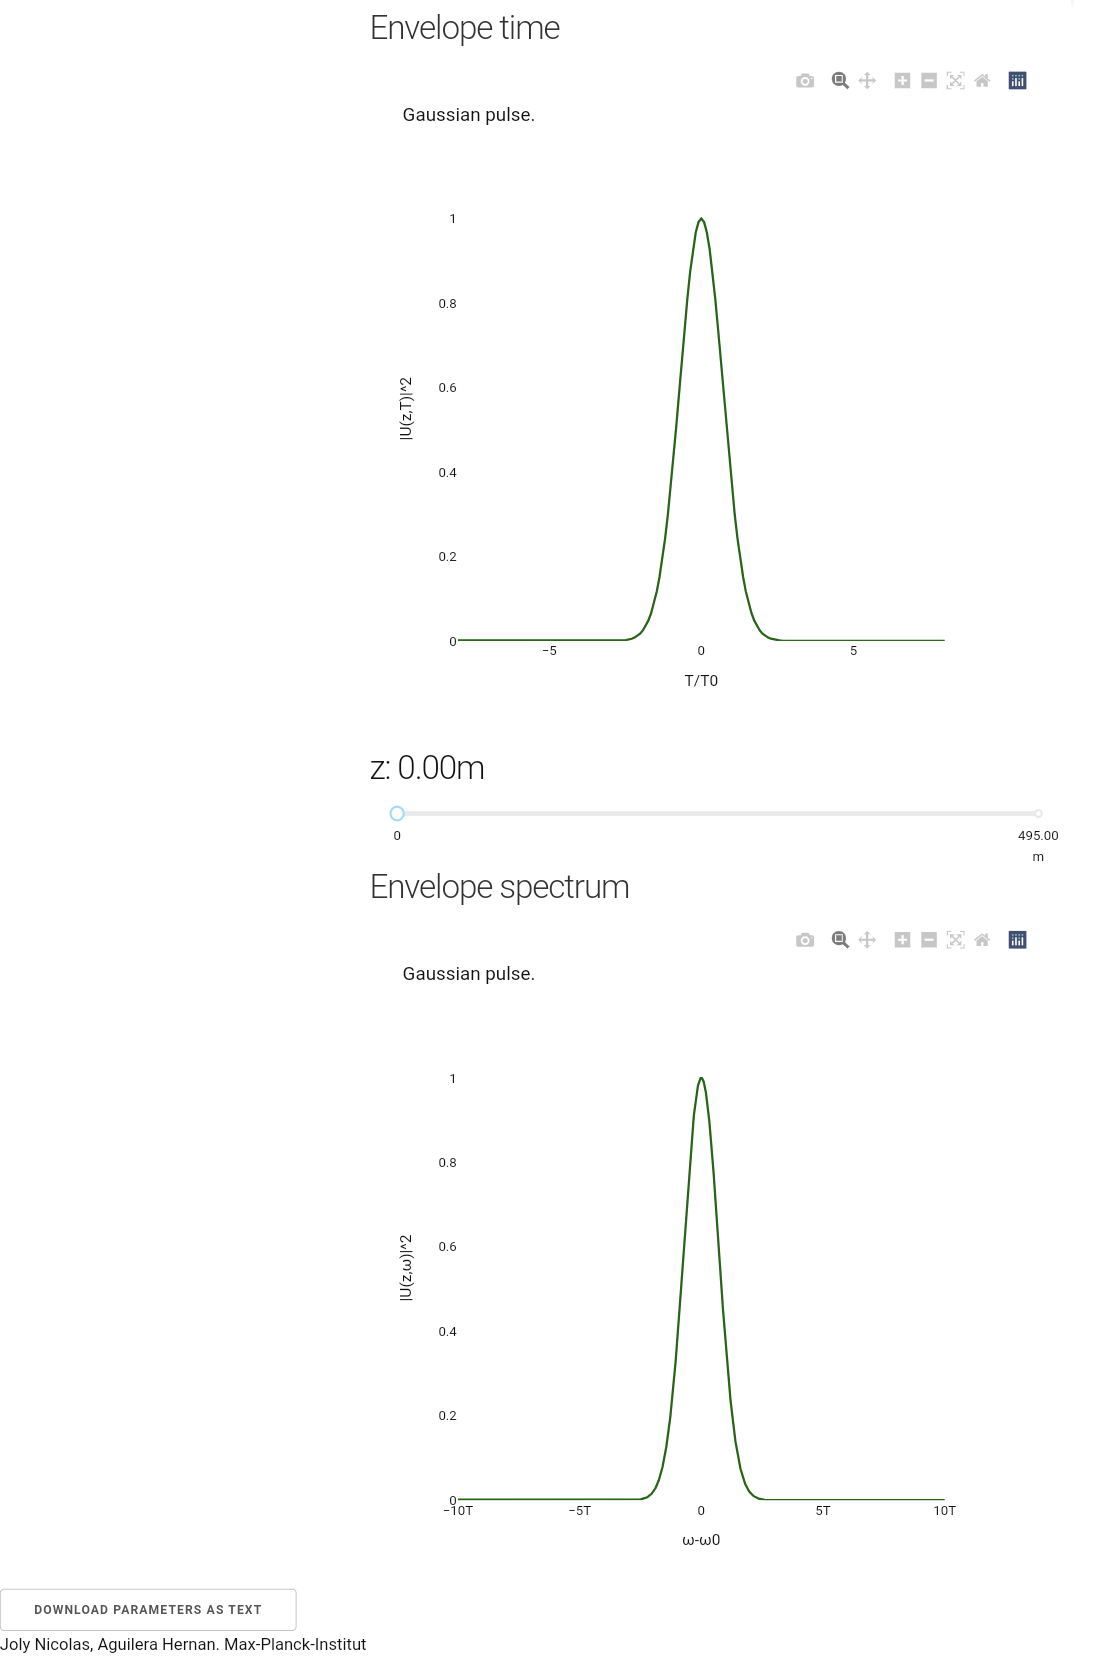
\includegraphics[width=1\textwidth]{figures/chap4/android_nlse2.png}
            \caption{Second part of the NLSE-app.}
            \label{fig:herokunlse2}
        \end{subfigure}}
        \end{tabular}
        \end{figure}
